\section{可视化子系统}
\addcontentsline{toe}{section}{{\currentchapter .3\ \ Visualization Subsystem}\numberline\,}
\label{sec:chap5-viz}

% almost finished
% indexed

联邦学习,乃至更广范围的机器学习领域,过程与结果的可视化是一个比较重要的方面,例如著名的深度学习软件包TensorFlow\cite{tensorflow}有配套的可视化工具TensorBoard\footnote{\url{https://www.tensorflow.org/tensorboard}},以及以Weight \& Biases\footnote{\url{https://wandb.ai/site}}为代表的专业化的机器学习全过程可视化工具,都对机器学习、深度学习等领域的研究起到了极大的促进作用。

联邦学习仿真系统\texttt{fl-sim}包含了为联邦学习量身定制的试验结果可视化面板系统\texttt{Panel}以及与之配套的试验日志系统。日志系统将试验过程中的模型评测数值同时以结构化的JSON文件,以及符合人类阅读习惯的文本文件的形式进行存储。可视化的面板系统\texttt{Panel}基于ipywidgets\footnote{\url{https://github.com/jupyter-widgets/ipywidgets}}开发,具备如下主要功能与特性
\begin{itemize}
    \item 自动从日志文件夹中搜索、列出所有完整试验的日志文件。
    \item 自动解析日志文件,完成模型评测数值曲线绘制。
    \item 支持绘制曲线 (图形) 平滑度、字体以及字体大小的动态调整。
    \item 支持绘制的图片以~PDF/SVG/PNG/JPEG/PS~等格式保存。
    \item 支持关键字形式的数值曲线合并,合并为均值曲线$\pm$误差界 (Error Bound) 的形式。误差界有4种选择,分别是标准差 (Standard Deviation, STD),样本均值的估计标准误差 (Standard Error of the Mean, SEM),四分位数 (Quartile)以及四分位距 (Interquartile Range, IQR)。
\end{itemize}

\begin{figure}[ht]
    \centering
    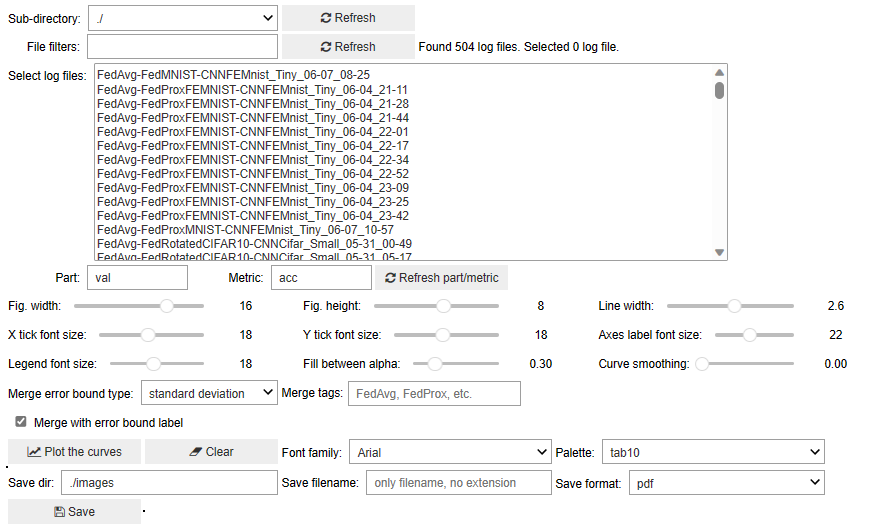
\includegraphics[width=\textwidth]{figures/panel-init.png}
    \caption{可视化的面板系统\texttt{Panel}的初始化界面}
    \label{fig:panel-init}
\end{figure}

图\ref{fig:panel-init}~是可视化的面板系统\texttt{Panel}的初始化界面。图\ref{fig:panel-init}~是可视化的面板系统\texttt{Panel}的使用示例,图中为使用\texttt{FedRotatedCIFAR10}数据集对\texttt{IFCA}算法\cite{Ghosh_2022_cfl}进行10轮试验 (5个不同的随机种子$\times$2种不同的数据增强组合),同时以联邦平均算法\texttt{FedAvg}以及局部训练作为对比方法的试验结果 (模型在验证集上的准确率)。可以清楚地看到\texttt{IFCA}算法相较于\texttt{FedAvg}算法在这一组试验上有明显的数值优势。

\begin{figure}[ht]
    \centering
    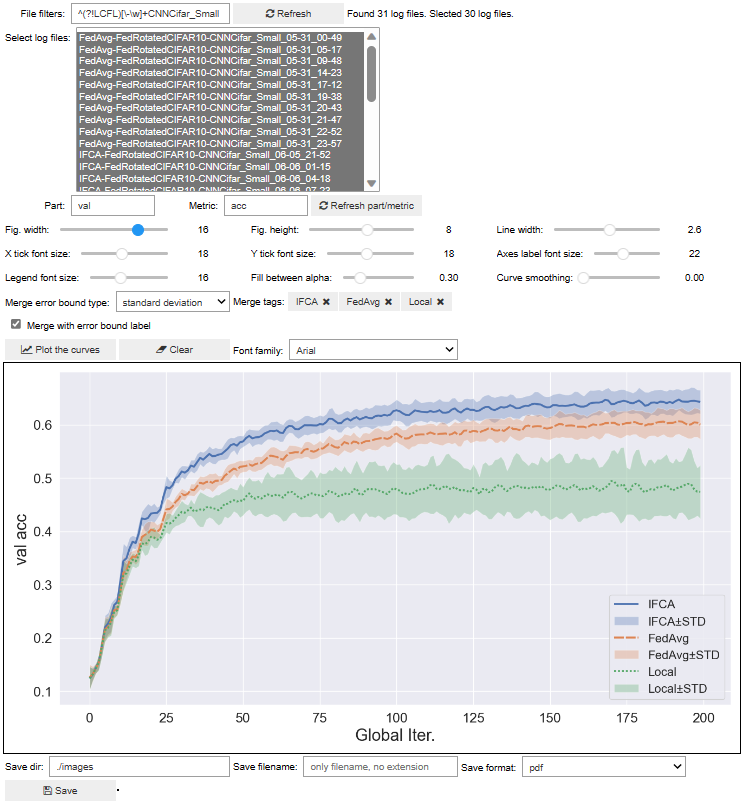
\includegraphics[width=\textwidth]{figures/panel-in-use.png}
    \caption{可视化的面板系统\texttt{Panel}的使用示例}
    \label{fig:panel-in-use}
\end{figure}
